\documentclass{article}
\usepackage[utf8]{inputenc}

\usepackage{natbib}
\usepackage{graphicx}
\usepackage{minted}

\begin{document}

%title
\begin{titlepage}
	\vspace{-20px}
	\begin{tabular}{l}
		\textsc{Blin} Sébastien\\
		\textsc{Drouin Viallard} Victor
	\end{tabular}
	\hfill \vspace{10px}
\includegraphics[scale=0.1]{uqac}\\
	\vfill
	\begin{center}
		\Huge{Université du Quebec à Chicoutimi}\\
		\vspace{1cm}
		\LARGE{Maîtrise professionnelle}\\
		\large{Parcours Informatique}\\
		\vspace{0.5cm}\hrule\vspace{0.5cm}
		\LARGE{\textbf{TP 2 8INF846}}\\
		\Large{Réalisation d'un solveur de Sudoku}
		\vspace{0.5cm}\hrule
		\vfill
		\vfill
	\end{center}
	\begin{flushleft}
		\Large{Sous l'encadrement de~:}\\
		\vspace{0.2cm}
		\large{\textsc{Bouchard} Kévin}
	\end{flushleft}
	\vfill
\end{titlepage}

\section{Introduction}
Le but de ce TP est de résoudre des sudokus en implémentant les algorithmes vu durant le cours \emph{Problèmes à satisfaction de contraintes}. Notre implémentation utilise les algorithmes AC3 pour la vérification des contraintes et une combinaison des algorithmes Backtracking et MRV pour la résolution en elle-même.


\section{Exécution du programme}
\subsection{Dépendances du projet}
Ce devoir a été développé en \emph{C++14} et a été testé sur des environnements
\emph{Linux} et \emph{Windows (dans le dossier bin)}. Pour compiler le
programme il vous faut~:
\begin{itemize}
    \item \emph{G++} (version 6 recommandée)
    \item La librairie \emph{SFML}
    \item \emph{Make}
\end{itemize}
\subsection{Compilation}
Pour compiler le programme, il suffit d'exécuter la commande \emph{make}. Un
binaire nommé \emph{sudokusolver} sera alors présent.

\subsection{Configuration et exécution}

Avant de lancer le programme, il faut tout d'abord un sudoku à résoudre. Pour ceci, il faut un fichier de la forme~:

\begin{verbatim}
,,3,,,,8,,,
,9,,4,,6,,5,,
4,,,,5,,,,9,
,7,,2,,3,,8,,
,,9,,,,4,,,
,1,,6,,9,,2,,
8,,,,2,,,,4,
,4,,7,,1,,6,,
,,7,,,,3,,,
\end{verbatim}

Puis pour éxécuter le programme
\begin{verbatim}
./sudokusolver sudoku_file
\end{verbatim}

Pour windows, il suffit d'ouvrir le programme \emph{cmd.exe}, de se rendre dans le dossier où se trouve l'éxécutable, et de taper~:
\begin{verbatim}
cd XXXXXXX\DOSSIERRENDU\bin\
sudokusolver.exe sudoku_file
\end{verbatim}

Nous proposons la série d'éxécution suivante~:
\begin{verbatim}
sudokusolver.exe sudoku1
sudokusolver.exe sudoku2
sudokusolver.exe sudoku3
\end{verbatim}


\section{Structure du programme}
\subsection{Structure générale}

La structure du programme est simple. Le programme possède une classe \emph{Sudoku} (qui contient un tableau de \emph{Cell}). Une \emph{Cell} est composée d'une valeur et de valeurs possibles. On donne ensuite le Sudoku à un objet \emph{Solver} qui se charge de la résolution.

\subsection{La résolution du sudoku}

\subsubsection{AC3}

Nous avons mis en place quelques algorithmes dans la classe \emph{Solver}. Le premier est l'algorithme \emph{AC3} pour vérifier la consistence des arcs. Ici, on considère chaque \emph{Cell} comme une variable ayant pour domaine ${1,2,3,...,N}$ ou $N$ est la taille du sudoku. Les contraintes sont ici propagées dans la méthode~:

\begin{minted}{c++}
	void Solver::updateSudokuConstraints();
\end{minted}

La contrainte propagée est qu'il ne doit pas y avoir 2 cases dans la même ligne, la même colonne, la même case avec la même valeur.

\subsubsection{Backtracking search + MRV}

Pour la résolution en elle-même on a choisit l'algorithme \emph{Backtracking search} amélioré avec \emph{MRV}. On peut le voir dans la méthode~:
\begin{minted}{c++}
	bool Solver::solve();
\end{minted}

La première étape est de trouver la variable ayant le plus grand nombre de contraintes (et donc le moins de valeurs possibles). Une fois que cette valeur est choisie, on remplace sa valeur dans le sudoku et on commence la construction de l'arbre de résolution. On a donc l'état actuel comme racine d'un noeud, et les possibilités de la MRV en branche. On choisit alors une branche qu'on essaye de résoudre. Si la résolution n'est pas possible, on retourne à l'état actuel et on tente de résoudre une autre branche. Si aucune branche ne peut-être résolue, alors le sudoku n'a pas de solutions. cf Fig \ref{fig:backtrackingmrv}

\begin{figure}[h]
	\begin{center}
			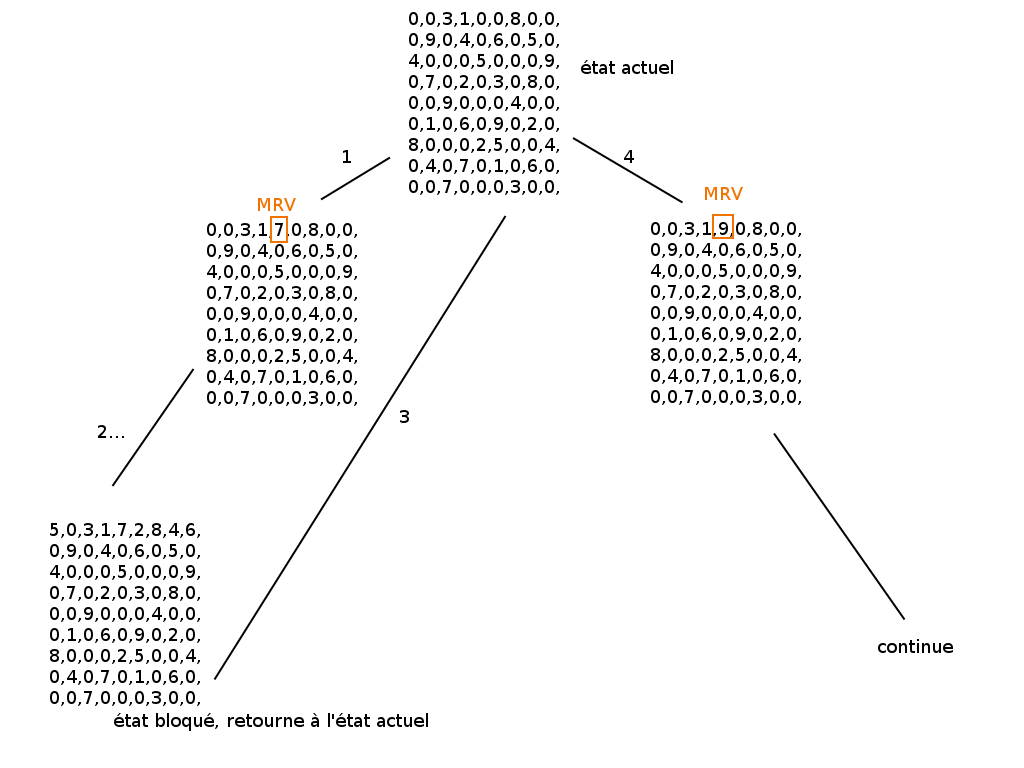
\includegraphics[scale=0.4]{backtrackingmrv}
		\caption{Backtracking + MRV}
		\label{fig:backtrackingmrv}
	\end{center}
\end{figure}

\subsubsection{Forward checking}

Enfin, un dernier point a été mis en place. L'exploration s'arrête lorsqu'une valeur n'a plus de valeurs possibles.

\section{Conclusion}
Ce TP a été l'occasion d'implémenter les différents algorithmes vus en cours comme le \emph{Backtracking + MRV} ou encore \emph{AC3} et donne un exemple de problèmes à satisfaction de contraintes.

\end{document}
